\documentclass[a4paper]{book}
\usepackage{makeidx}
\usepackage{graphicx}
\usepackage{multicol}
\usepackage{float}
\usepackage{listings}
\usepackage{color}
\usepackage{ifthen}
\usepackage[table]{xcolor}
\usepackage{textcomp}
\usepackage{alltt}
\usepackage{ifpdf}
\ifpdf
\usepackage[pdftex,
            pagebackref=true,
            colorlinks=true,
            linkcolor=blue,
            unicode
           ]{hyperref}
\else
\usepackage[ps2pdf,
            pagebackref=true,
            colorlinks=true,
            linkcolor=blue,
            unicode
           ]{hyperref}
\usepackage{pspicture}
\fi
\usepackage[utf8]{inputenc}
\usepackage{mathptmx}
\usepackage[scaled=.90]{helvet}
\usepackage{courier}
\usepackage{doxygen}
\lstset{language=C++,inputencoding=utf8,basicstyle=\footnotesize,breaklines=true,breakatwhitespace=true,tabsize=8,numbers=left }
\makeindex
\setcounter{tocdepth}{3}
\renewcommand{\footrulewidth}{0.4pt}
\begin{document}
\hypersetup{pageanchor=false}
\begin{titlepage}
\vspace*{7cm}
\begin{center}
{\Large Baralho }\\
\vspace*{1cm}
{\large Generated by Doxygen 1.7.3}\\
\vspace*{0.5cm}
{\small Wed May 16 2012 22:41:07}\\
\end{center}
\end{titlepage}
\clearemptydoublepage
\pagenumbering{roman}
\tableofcontents
\clearemptydoublepage
\pagenumbering{arabic}
\hypersetup{pageanchor=true}
\chapter{Namespace Index}
\section{Packages}
Here are the packages with brief descriptions (if available):\begin{DoxyCompactList}
\item\contentsline{section}{\hyperlink{namespace_exec}{Exec} }{\pageref{namespace_exec}}{}
\item\contentsline{section}{\hyperlink{namespace_jogo}{Jogo} }{\pageref{namespace_jogo}}{}
\end{DoxyCompactList}

\chapter{Class Index}
\section{Class Hierarchy}
This inheritance list is sorted roughly, but not completely, alphabetically:\begin{DoxyCompactList}
\item \contentsline{section}{Baralho.Baralho}{\pageref{class_baralho_1_1_baralho}}{}
\item \contentsline{section}{Baralho.Carta}{\pageref{class_baralho_1_1_carta}}{}
\item \contentsline{section}{Exceções.CartaInexistenteException}{\pageref{class_exce_xC3_xA7_xC3_xB5es_1_1_carta_inexistente_exception}}{}
\item \contentsline{section}{Exceções.CartaInvalidaException}{\pageref{class_exce_xC3_xA7_xC3_xB5es_1_1_carta_invalida_exception}}{}
\item \contentsline{section}{Baralho.ComparaCartas}{\pageref{interface_baralho_1_1_compara_cartas}}{}
\begin{DoxyCompactList}
\item \contentsline{section}{Baralho.ComparacaoSimples}{\pageref{class_baralho_1_1_comparacao_simples}}{}
\end{DoxyCompactList}
\item \contentsline{section}{Baralho.Monte}{\pageref{class_baralho_1_1_monte}}{}
\begin{DoxyCompactList}
\item \contentsline{section}{Baralho.MonteComum}{\pageref{class_baralho_1_1_monte_comum}}{}
\item \contentsline{section}{Baralho.MonteDescarte}{\pageref{class_baralho_1_1_monte_descarte}}{}
\end{DoxyCompactList}
\item \contentsline{section}{Exceções.SequenciaInvalidaException}{\pageref{class_exce_xC3_xA7_xC3_xB5es_1_1_sequencia_invalida_exception}}{}
\end{DoxyCompactList}

\chapter{Class Index}
\section{Estruturas de Dados}
Aqui estão as estruturas de dados, uniões e suas respectivas descrições:\begin{DoxyCompactList}
\item\contentsline{section}{\hyperlink{structnodo}{nodo} }{\pageref{structnodo}}{}
\end{DoxyCompactList}

\chapter{File Index}
\section{File List}
Here is a list of all files with brief descriptions:\begin{DoxyCompactList}
\item\contentsline{section}{aula/111450026/Trabalho Baralho/Truco/src/Exec/\hyperlink{_main_8java}{Main.java} }{\pageref{_main_8java}}{}
\item\contentsline{section}{aula/111450026/Trabalho Baralho/Truco/src/Jogo/\hyperlink{_comparacao_truco_8java}{ComparacaoTruco.java} }{\pageref{_comparacao_truco_8java}}{}
\item\contentsline{section}{aula/111450026/Trabalho Baralho/Truco/src/Jogo/\hyperlink{_jogador_8java}{Jogador.java} }{\pageref{_jogador_8java}}{}
\item\contentsline{section}{aula/111450026/Trabalho Baralho/Truco/src/Jogo/\hyperlink{_jogo_8java}{Jogo.java} }{\pageref{_jogo_8java}}{}
\end{DoxyCompactList}

\chapter{Namespace Documentation}
\hypertarget{namespace_baralho}{
\section{Package Baralho}
\label{namespace_baralho}\index{Baralho@{Baralho}}
}
\subsection*{Classes}
\begin{DoxyCompactItemize}
\item 
class \hyperlink{class_baralho_1_1_baralho}{Baralho}
\item 
class \hyperlink{class_baralho_1_1_carta}{Carta}
\item 
class \hyperlink{class_baralho_1_1_comparacao_simples}{ComparacaoSimples}
\item 
interface \hyperlink{interface_baralho_1_1_compara_cartas}{ComparaCartas}
\item 
class \hyperlink{class_baralho_1_1_monte}{Monte}
\item 
class \hyperlink{class_baralho_1_1_monte_comum}{MonteComum}
\item 
class \hyperlink{class_baralho_1_1_monte_descarte}{MonteDescarte}
\end{DoxyCompactItemize}
\subsection*{Enumerations}
\begin{DoxyCompactItemize}
\item 
enum \hyperlink{namespace_baralho_ab887857dcb81ef6672322ce80039b905}{Naipe} \{ \hyperlink{namespace_baralho_ab887857dcb81ef6672322ce80039b905}{OUROS}, 
\hyperlink{namespace_baralho_ab887857dcb81ef6672322ce80039b905}{peso}, 
\hyperlink{namespace_baralho_ab887857dcb81ef6672322ce80039b905}{peso}, 
\hyperlink{namespace_baralho_ab887857dcb81ef6672322ce80039b905}{peso}
 \}
\end{DoxyCompactItemize}


\subsection{Enumeration Type Documentation}
\hypertarget{namespace_baralho_ab887857dcb81ef6672322ce80039b905}{
\index{Baralho@{Baralho}!Naipe@{Naipe}}
\index{Naipe@{Naipe}!Baralho@{Baralho}}
\subsubsection[{Naipe}]{\setlength{\rightskip}{0pt plus 5cm}enum {\bf Baralho::Naipe}}}
\label{namespace_baralho_ab887857dcb81ef6672322ce80039b905}
\begin{Desc}
\item[Enumerator: ]\par
\begin{description}
\index{OUROS@{OUROS}!Baralho@{Baralho}}\index{Baralho@{Baralho}!OUROS@{OUROS}}\item[{\em 
\hypertarget{namespace_baralho_ab887857dcb81ef6672322ce80039b905}{
OUROS}
\label{namespace_baralho_ab887857dcb81ef6672322ce80039b905}
}]\index{peso@{peso}!Baralho@{Baralho}}\index{Baralho@{Baralho}!peso@{peso}}\item[{\em 
\hypertarget{namespace_baralho_ab887857dcb81ef6672322ce80039b905}{
peso}
\label{namespace_baralho_ab887857dcb81ef6672322ce80039b905}
}]\index{peso@{peso}!Baralho@{Baralho}}\index{Baralho@{Baralho}!peso@{peso}}\item[{\em 
\hypertarget{namespace_baralho_ab887857dcb81ef6672322ce80039b905}{
peso}
\label{namespace_baralho_ab887857dcb81ef6672322ce80039b905}
}]\index{peso@{peso}!Baralho@{Baralho}}\index{Baralho@{Baralho}!peso@{peso}}\item[{\em 
\hypertarget{namespace_baralho_ab887857dcb81ef6672322ce80039b905}{
peso}
\label{namespace_baralho_ab887857dcb81ef6672322ce80039b905}
}]\end{description}
\end{Desc}


\hypertarget{namespace_exce_xC3_xA7_xC3_xB5es}{
\section{Package Exceções}
\label{namespace_exce_xC3_xA7_xC3_xB5es}\index{Exceções@{Exceções}}
}
\subsection*{Classes}
\begin{DoxyCompactItemize}
\item 
class \hyperlink{class_exce_xC3_xA7_xC3_xB5es_1_1_carta_inexistente_exception}{CartaInexistenteException}
\item 
class \hyperlink{class_exce_xC3_xA7_xC3_xB5es_1_1_carta_invalida_exception}{CartaInvalidaException}
\item 
class \hyperlink{class_exce_xC3_xA7_xC3_xB5es_1_1_sequencia_invalida_exception}{SequenciaInvalidaException}
\end{DoxyCompactItemize}

\chapter{Class Documentation}
\hypertarget{class_baralho_1_1_baralho}{
\section{Baralho.Baralho Class Reference}
\label{class_baralho_1_1_baralho}\index{Baralho::Baralho@{Baralho::Baralho}}
}
\subsection*{Public Member Functions}
\begin{DoxyCompactItemize}
\item 
\hyperlink{class_baralho_1_1_baralho_ab88f90bd08144f150e97b45bd63eadfd}{Baralho} (\hyperlink{class_baralho_1_1_monte}{Monte} montePrincipal, \hyperlink{class_baralho_1_1_monte_descarte}{MonteDescarte} monteDescarte)
\item 
\hyperlink{class_baralho_1_1_baralho_a039c014d8bf91ceda3b003a1ee4d2418}{Baralho} (\hyperlink{class_baralho_1_1_monte}{Monte} montePrincipal, \hyperlink{class_baralho_1_1_monte_descarte}{MonteDescarte} monteDescarte, \hyperlink{interface_baralho_1_1_compara_cartas}{ComparaCartas} formaComparacao)
\item 
\hyperlink{class_baralho_1_1_baralho_a749ad25fed6cc2df5be8e1b2d8db5881}{Baralho} (\hyperlink{class_baralho_1_1_monte}{Monte} montePrincipal, \hyperlink{class_baralho_1_1_monte_descarte}{MonteDescarte} monteDescarte, \hyperlink{interface_baralho_1_1_compara_cartas}{ComparaCartas} formaComparacao, List$<$ Integer $>$ sequencia)  throws SequenciaInvalidaException
\item 
void \hyperlink{class_baralho_1_1_baralho_ae7ce198ebeadf6c0b3fb5ad109873f1c}{reiniciarBaralho} ()
\item 
void \hyperlink{class_baralho_1_1_baralho_a5d5b81ee3a6b48f6a99117172d23a24a}{reiniciarBaralho} (List$<$ Integer $>$ sequencia, \hyperlink{interface_baralho_1_1_compara_cartas}{ComparaCartas} comparacao)  throws SequenciaInvalidaException
\item 
void \hyperlink{class_baralho_1_1_baralho_a97297169abcfe6cdfe434b42bb121d5d}{setComparacao} (\hyperlink{interface_baralho_1_1_compara_cartas}{ComparaCartas} cc)
\item 
void \hyperlink{class_baralho_1_1_baralho_a50716e1d93b3ed27800ac62b7b9e8b8a}{embaralhar} ()
\item 
void \hyperlink{class_baralho_1_1_baralho_a6839090e52620e5b665a12aceeba06f6}{cortar} (int ini, int fim)  throws CartaInexistenteException
\item 
\hyperlink{class_baralho_1_1_carta}{Carta} \hyperlink{class_baralho_1_1_baralho_a88c1b1eec22e717be39227ed2ceb9490}{retirarCartaDoInicio} ()  throws CartaInexistenteException
\item 
\hyperlink{class_baralho_1_1_carta}{Carta} \hyperlink{class_baralho_1_1_baralho_a8441347c4eb47a0ba0f3bfbdfca59a9c}{retirarCartaDoFim} ()  throws CartaInexistenteException 
\item 
void \hyperlink{class_baralho_1_1_baralho_a9df1c0a9c5c6c227b36e434248d5698d}{moverDoInicioParaFim} ()  throws CartaInexistenteException 
\item 
boolean \hyperlink{class_baralho_1_1_baralho_ad95b8caaaf2602be21923a9c02ab741f}{descartar} (\hyperlink{class_baralho_1_1_carta}{Carta} carta)
\item 
\hyperlink{class_baralho_1_1_carta}{Carta} \hyperlink{class_baralho_1_1_baralho_ad6ceed72b137e5bf5490af7dcd282648}{retirarCartaDoDescarte} (int pos)  throws CartaInexistenteException 
\item 
void \hyperlink{class_baralho_1_1_baralho_a9a20256555c03889f244ce40957ae7f8}{verCartaDoDescarte} (int pos)  throws CartaInexistenteException 
\item 
int \hyperlink{class_baralho_1_1_baralho_ac382a9e91f65da63c8e3fac26eba6225}{tamanho} ()
\item 
int \hyperlink{class_baralho_1_1_baralho_aace43f8f3dbbca74e2e2b5083ec3f305}{tamanhoMontePrincipal} ()
\item 
int \hyperlink{class_baralho_1_1_baralho_a2c293b134d1b685b19e46376097c02b8}{tamanhoMonteDescarte} ()
\end{DoxyCompactItemize}


\subsection{Detailed Description}
Classe que representa o baralho. O baralho conta com dois montes: \hyperlink{class_baralho_1_1_monte}{Monte} principal: monte inicial do baralho. O monte que sofre o corte e onde se compram as cartas. \hyperlink{class_baralho_1_1_monte}{Monte} de descarte: monte para vão as cartas descartadas pelos usuários do baralho. \begin{DoxyAuthor}{Author}
Rafael 
\end{DoxyAuthor}


\subsection{Constructor \& Destructor Documentation}
\hypertarget{class_baralho_1_1_baralho_ab88f90bd08144f150e97b45bd63eadfd}{
\index{Baralho::Baralho@{Baralho::Baralho}!Baralho@{Baralho}}
\index{Baralho@{Baralho}!Baralho::Baralho@{Baralho::Baralho}}
\subsubsection[{Baralho}]{\setlength{\rightskip}{0pt plus 5cm}Baralho.Baralho.Baralho (
\begin{DoxyParamCaption}
\item[{{\bf Monte}}]{montePrincipal, }
\item[{{\bf MonteDescarte}}]{monteDescarte}
\end{DoxyParamCaption}
)}}
\label{class_baralho_1_1_baralho_ab88f90bd08144f150e97b45bd63eadfd}

\begin{DoxyParams}{Parameters}
{\em montePrincipal} & -\/ \hyperlink{class_baralho_1_1_monte}{Monte} de compra. \\
\hline
{\em monteDescarte} & -\/ \hyperlink{class_baralho_1_1_monte}{Monte} de descarte. \\
\hline
\end{DoxyParams}
\hypertarget{class_baralho_1_1_baralho_a039c014d8bf91ceda3b003a1ee4d2418}{
\index{Baralho::Baralho@{Baralho::Baralho}!Baralho@{Baralho}}
\index{Baralho@{Baralho}!Baralho::Baralho@{Baralho::Baralho}}
\subsubsection[{Baralho}]{\setlength{\rightskip}{0pt plus 5cm}Baralho.Baralho.Baralho (
\begin{DoxyParamCaption}
\item[{{\bf Monte}}]{montePrincipal, }
\item[{{\bf MonteDescarte}}]{monteDescarte, }
\item[{{\bf ComparaCartas}}]{formaComparacao}
\end{DoxyParamCaption}
)}}
\label{class_baralho_1_1_baralho_a039c014d8bf91ceda3b003a1ee4d2418}

\begin{DoxyParams}{Parameters}
{\em montePrincipal} & -\/ \hyperlink{class_baralho_1_1_monte}{Monte} de compra. \\
\hline
{\em monteDescarte} & -\/ \hyperlink{class_baralho_1_1_monte}{Monte} de descarte. \\
\hline
{\em formaComparacao} & -\/ Forma de comparação das cartas. \\
\hline
\end{DoxyParams}
\hypertarget{class_baralho_1_1_baralho_a749ad25fed6cc2df5be8e1b2d8db5881}{
\index{Baralho::Baralho@{Baralho::Baralho}!Baralho@{Baralho}}
\index{Baralho@{Baralho}!Baralho::Baralho@{Baralho::Baralho}}
\subsubsection[{Baralho}]{\setlength{\rightskip}{0pt plus 5cm}Baralho.Baralho.Baralho (
\begin{DoxyParamCaption}
\item[{{\bf Monte}}]{montePrincipal, }
\item[{{\bf MonteDescarte}}]{monteDescarte, }
\item[{{\bf ComparaCartas}}]{formaComparacao, }
\item[{List$<$ Integer $>$}]{sequencia}
\end{DoxyParamCaption}
)  throws {\bf SequenciaInvalidaException}}}
\label{class_baralho_1_1_baralho_a749ad25fed6cc2df5be8e1b2d8db5881}

\begin{DoxyParams}{Parameters}
{\em montePrincipal} & \hyperlink{class_baralho_1_1_monte}{Monte} de compra. \\
\hline
{\em monteDescarte} & \hyperlink{class_baralho_1_1_monte}{Monte} de descarte. \\
\hline
{\em formaComparacao} & Forma de comparação de cartas. \\
\hline
{\em sequencia} & Sequência contendo os valores das cartas que serão inseridas no baralho (entre 1 e 13). \\
\hline
\end{DoxyParams}

\begin{DoxyExceptions}{Exceptions}
{\em SequenciaInvalidaException} & Caso a sequência contenha valores menores que 0 ou maiores que 13. \\
\hline
\end{DoxyExceptions}


\subsection{Member Function Documentation}
\hypertarget{class_baralho_1_1_baralho_a6839090e52620e5b665a12aceeba06f6}{
\index{Baralho::Baralho@{Baralho::Baralho}!cortar@{cortar}}
\index{cortar@{cortar}!Baralho::Baralho@{Baralho::Baralho}}
\subsubsection[{cortar}]{\setlength{\rightskip}{0pt plus 5cm}void Baralho.Baralho.cortar (
\begin{DoxyParamCaption}
\item[{int}]{ini, }
\item[{int}]{fim}
\end{DoxyParamCaption}
)  throws {\bf CartaInexistenteException}}}
\label{class_baralho_1_1_baralho_a6839090e52620e5b665a12aceeba06f6}
Faz um corte no baralho, ou seja, retira um conjunto de cartas do baralho e as passa para o topo. 
\begin{DoxyParams}{Parameters}
{\em ini} & Posição de onde começa o conjunto a ser retirado. \\
\hline
{\em fim} & Posição de onde termina o conjunto a ser retirado. \\
\hline
\end{DoxyParams}

\begin{DoxyExceptions}{Exceptions}
{\em CartaInexistenteException} & -\/ Caso alguma das posições (inicial ou final) especificada aponte para uma carta que não existe no monte. \\
\hline
\end{DoxyExceptions}
\hypertarget{class_baralho_1_1_baralho_ad95b8caaaf2602be21923a9c02ab741f}{
\index{Baralho::Baralho@{Baralho::Baralho}!descartar@{descartar}}
\index{descartar@{descartar}!Baralho::Baralho@{Baralho::Baralho}}
\subsubsection[{descartar}]{\setlength{\rightskip}{0pt plus 5cm}boolean Baralho.Baralho.descartar (
\begin{DoxyParamCaption}
\item[{{\bf Carta}}]{carta}
\end{DoxyParamCaption}
)}}
\label{class_baralho_1_1_baralho_ad95b8caaaf2602be21923a9c02ab741f}
Adiciona uma carta ao monte de descarte. 
\begin{DoxyParams}{Parameters}
{\em carta} & -\/ \hyperlink{class_baralho_1_1_carta}{Carta} a ser adicionada ao descarte. \\
\hline
\end{DoxyParams}
\begin{DoxyReturn}{Returns}
true se a carta foi adicionada ou false caso contrário. 
\end{DoxyReturn}
\hypertarget{class_baralho_1_1_baralho_a50716e1d93b3ed27800ac62b7b9e8b8a}{
\index{Baralho::Baralho@{Baralho::Baralho}!embaralhar@{embaralhar}}
\index{embaralhar@{embaralhar}!Baralho::Baralho@{Baralho::Baralho}}
\subsubsection[{embaralhar}]{\setlength{\rightskip}{0pt plus 5cm}void Baralho.Baralho.embaralhar (
\begin{DoxyParamCaption}
{}
\end{DoxyParamCaption}
)}}
\label{class_baralho_1_1_baralho_a50716e1d93b3ed27800ac62b7b9e8b8a}
Embaralha as cartas do baralho. \hypertarget{class_baralho_1_1_baralho_a9df1c0a9c5c6c227b36e434248d5698d}{
\index{Baralho::Baralho@{Baralho::Baralho}!moverDoInicioParaFim@{moverDoInicioParaFim}}
\index{moverDoInicioParaFim@{moverDoInicioParaFim}!Baralho::Baralho@{Baralho::Baralho}}
\subsubsection[{moverDoInicioParaFim}]{\setlength{\rightskip}{0pt plus 5cm}void Baralho.Baralho.moverDoInicioParaFim (
\begin{DoxyParamCaption}
{}
\end{DoxyParamCaption}
)  throws {\bf CartaInexistenteException} }}
\label{class_baralho_1_1_baralho_a9df1c0a9c5c6c227b36e434248d5698d}
Retira uma carta do topo do baralho e a passa para o início do baralho. 
\begin{DoxyExceptions}{Exceptions}
{\em CartaInexistenteException} & -\/ Caso não haja mais cartas no monte principal. \\
\hline
\end{DoxyExceptions}
\hypertarget{class_baralho_1_1_baralho_a5d5b81ee3a6b48f6a99117172d23a24a}{
\index{Baralho::Baralho@{Baralho::Baralho}!reiniciarBaralho@{reiniciarBaralho}}
\index{reiniciarBaralho@{reiniciarBaralho}!Baralho::Baralho@{Baralho::Baralho}}
\subsubsection[{reiniciarBaralho}]{\setlength{\rightskip}{0pt plus 5cm}void Baralho.Baralho.reiniciarBaralho (
\begin{DoxyParamCaption}
\item[{List$<$ Integer $>$}]{sequencia, }
\item[{{\bf ComparaCartas}}]{comparacao}
\end{DoxyParamCaption}
)  throws {\bf SequenciaInvalidaException}}}
\label{class_baralho_1_1_baralho_a5d5b81ee3a6b48f6a99117172d23a24a}
Elimina as carta dos monte e inicialize o baralho novamente (initalize()). 
\begin{DoxyParams}{Parameters}
{\em sequencia} & Sequência contendo os valores das cartas que serão inseridas no baralho (Entre 1 e 13). \\
\hline
{\em comparacao} & Foma de comparação das cartas. \\
\hline
\end{DoxyParams}

\begin{DoxyExceptions}{Exceptions}
{\em SequenciaInvalidaException} & Caso a sequência contenha valores menores que 0 ou maiores que 13. \\
\hline
\end{DoxyExceptions}
\hypertarget{class_baralho_1_1_baralho_ae7ce198ebeadf6c0b3fb5ad109873f1c}{
\index{Baralho::Baralho@{Baralho::Baralho}!reiniciarBaralho@{reiniciarBaralho}}
\index{reiniciarBaralho@{reiniciarBaralho}!Baralho::Baralho@{Baralho::Baralho}}
\subsubsection[{reiniciarBaralho}]{\setlength{\rightskip}{0pt plus 5cm}void Baralho.Baralho.reiniciarBaralho (
\begin{DoxyParamCaption}
{}
\end{DoxyParamCaption}
)}}
\label{class_baralho_1_1_baralho_ae7ce198ebeadf6c0b3fb5ad109873f1c}
Elimina as cartas dos montes e inicializa o baralho novamente (initialize()). \hypertarget{class_baralho_1_1_baralho_ad6ceed72b137e5bf5490af7dcd282648}{
\index{Baralho::Baralho@{Baralho::Baralho}!retirarCartaDoDescarte@{retirarCartaDoDescarte}}
\index{retirarCartaDoDescarte@{retirarCartaDoDescarte}!Baralho::Baralho@{Baralho::Baralho}}
\subsubsection[{retirarCartaDoDescarte}]{\setlength{\rightskip}{0pt plus 5cm}{\bf Carta} Baralho.Baralho.retirarCartaDoDescarte (
\begin{DoxyParamCaption}
\item[{int}]{pos}
\end{DoxyParamCaption}
)  throws {\bf CartaInexistenteException} }}
\label{class_baralho_1_1_baralho_ad6ceed72b137e5bf5490af7dcd282648}
Retira uma carta do monte de descarte. 
\begin{DoxyParams}{Parameters}
{\em pos} & -\/ Posição do monte de descarte de onde a carta será retirada. \\
\hline
\end{DoxyParams}
\begin{DoxyReturn}{Returns}
A carta, caso a posição especificada aponte para uma carta do monte. 
\end{DoxyReturn}

\begin{DoxyExceptions}{Exceptions}
{\em CartaInexistenteException} & -\/ Caso a posição especificada não aponte para uma carta no monte. \\
\hline
\end{DoxyExceptions}
\hypertarget{class_baralho_1_1_baralho_a8441347c4eb47a0ba0f3bfbdfca59a9c}{
\index{Baralho::Baralho@{Baralho::Baralho}!retirarCartaDoFim@{retirarCartaDoFim}}
\index{retirarCartaDoFim@{retirarCartaDoFim}!Baralho::Baralho@{Baralho::Baralho}}
\subsubsection[{retirarCartaDoFim}]{\setlength{\rightskip}{0pt plus 5cm}{\bf Carta} Baralho.Baralho.retirarCartaDoFim (
\begin{DoxyParamCaption}
{}
\end{DoxyParamCaption}
)  throws {\bf CartaInexistenteException} }}
\label{class_baralho_1_1_baralho_a8441347c4eb47a0ba0f3bfbdfca59a9c}
Retira uma carta do topo do monte principal. \begin{DoxyReturn}{Returns}
\hyperlink{class_baralho_1_1_carta}{Carta} -\/ \hyperlink{class_baralho_1_1_carta}{Carta} retidada do topo do monte principal 
\end{DoxyReturn}

\begin{DoxyExceptions}{Exceptions}
{\em CartaInexistenteException} & -\/ Caso não haja mais cartas no monte principal. \\
\hline
\end{DoxyExceptions}
\hypertarget{class_baralho_1_1_baralho_a88c1b1eec22e717be39227ed2ceb9490}{
\index{Baralho::Baralho@{Baralho::Baralho}!retirarCartaDoInicio@{retirarCartaDoInicio}}
\index{retirarCartaDoInicio@{retirarCartaDoInicio}!Baralho::Baralho@{Baralho::Baralho}}
\subsubsection[{retirarCartaDoInicio}]{\setlength{\rightskip}{0pt plus 5cm}{\bf Carta} Baralho.Baralho.retirarCartaDoInicio (
\begin{DoxyParamCaption}
{}
\end{DoxyParamCaption}
)  throws {\bf CartaInexistenteException}}}
\label{class_baralho_1_1_baralho_a88c1b1eec22e717be39227ed2ceb9490}
Retira uma carta do início do monte principal. \begin{DoxyReturn}{Returns}
\hyperlink{class_baralho_1_1_carta}{Carta} -\/ \hyperlink{class_baralho_1_1_carta}{Carta} retirada do início do baralho. 
\end{DoxyReturn}

\begin{DoxyExceptions}{Exceptions}
{\em CartaInexistenteException} & -\/ Caso não haja mais cartas no monte principal. \\
\hline
\end{DoxyExceptions}
\hypertarget{class_baralho_1_1_baralho_a97297169abcfe6cdfe434b42bb121d5d}{
\index{Baralho::Baralho@{Baralho::Baralho}!setComparacao@{setComparacao}}
\index{setComparacao@{setComparacao}!Baralho::Baralho@{Baralho::Baralho}}
\subsubsection[{setComparacao}]{\setlength{\rightskip}{0pt plus 5cm}void Baralho.Baralho.setComparacao (
\begin{DoxyParamCaption}
\item[{{\bf ComparaCartas}}]{cc}
\end{DoxyParamCaption}
)}}
\label{class_baralho_1_1_baralho_a97297169abcfe6cdfe434b42bb121d5d}
Configura a forma de comparação das cartas do baralho. 
\begin{DoxyParams}{Parameters}
{\em cc} & Forma de comparação das cartas. \\
\hline
\end{DoxyParams}
\hypertarget{class_baralho_1_1_baralho_ac382a9e91f65da63c8e3fac26eba6225}{
\index{Baralho::Baralho@{Baralho::Baralho}!tamanho@{tamanho}}
\index{tamanho@{tamanho}!Baralho::Baralho@{Baralho::Baralho}}
\subsubsection[{tamanho}]{\setlength{\rightskip}{0pt plus 5cm}int Baralho.Baralho.tamanho (
\begin{DoxyParamCaption}
{}
\end{DoxyParamCaption}
)}}
\label{class_baralho_1_1_baralho_ac382a9e91f65da63c8e3fac26eba6225}
Retorna o tamanho do baralho. O tamanho do baralho é dado pela soma do tamanho do monte principal com o tamanho do monte de descarte. \begin{DoxyReturn}{Returns}
Tamanho do baralho. 
\end{DoxyReturn}
\hypertarget{class_baralho_1_1_baralho_a2c293b134d1b685b19e46376097c02b8}{
\index{Baralho::Baralho@{Baralho::Baralho}!tamanhoMonteDescarte@{tamanhoMonteDescarte}}
\index{tamanhoMonteDescarte@{tamanhoMonteDescarte}!Baralho::Baralho@{Baralho::Baralho}}
\subsubsection[{tamanhoMonteDescarte}]{\setlength{\rightskip}{0pt plus 5cm}int Baralho.Baralho.tamanhoMonteDescarte (
\begin{DoxyParamCaption}
{}
\end{DoxyParamCaption}
)}}
\label{class_baralho_1_1_baralho_a2c293b134d1b685b19e46376097c02b8}
Retorna o tamanho do mont de descarte (quantidade de cartas). \begin{DoxyReturn}{Returns}
Tamanho do monte de descarte. 
\end{DoxyReturn}
\hypertarget{class_baralho_1_1_baralho_aace43f8f3dbbca74e2e2b5083ec3f305}{
\index{Baralho::Baralho@{Baralho::Baralho}!tamanhoMontePrincipal@{tamanhoMontePrincipal}}
\index{tamanhoMontePrincipal@{tamanhoMontePrincipal}!Baralho::Baralho@{Baralho::Baralho}}
\subsubsection[{tamanhoMontePrincipal}]{\setlength{\rightskip}{0pt plus 5cm}int Baralho.Baralho.tamanhoMontePrincipal (
\begin{DoxyParamCaption}
{}
\end{DoxyParamCaption}
)}}
\label{class_baralho_1_1_baralho_aace43f8f3dbbca74e2e2b5083ec3f305}
Retorna o tamanho do monte principal (quantidade de cartas). \begin{DoxyReturn}{Returns}
Tamanho do monte principal. 
\end{DoxyReturn}
\hypertarget{class_baralho_1_1_baralho_a9a20256555c03889f244ce40957ae7f8}{
\index{Baralho::Baralho@{Baralho::Baralho}!verCartaDoDescarte@{verCartaDoDescarte}}
\index{verCartaDoDescarte@{verCartaDoDescarte}!Baralho::Baralho@{Baralho::Baralho}}
\subsubsection[{verCartaDoDescarte}]{\setlength{\rightskip}{0pt plus 5cm}void Baralho.Baralho.verCartaDoDescarte (
\begin{DoxyParamCaption}
\item[{int}]{pos}
\end{DoxyParamCaption}
)  throws {\bf CartaInexistenteException} }}
\label{class_baralho_1_1_baralho_a9a20256555c03889f244ce40957ae7f8}
Exibe uma carta do monte de descarte. 
\begin{DoxyParams}{Parameters}
{\em pos} & -\/ Posição do monte de descarte que aponta para a carta a ser exibida. \\
\hline
\end{DoxyParams}

\begin{DoxyExceptions}{Exceptions}
{\em CartaInexistenteException} & -\/ Caso a posição especificada não aponte para uma carta no monte. \\
\hline
\end{DoxyExceptions}


The documentation for this class was generated from the following file:\begin{DoxyCompactItemize}
\item 
aula/111450026/Trabalho Baralho/Baralho/src/Baralho/\hyperlink{_baralho_8java}{Baralho.java}\end{DoxyCompactItemize}

\hypertarget{class_baralho_1_1_carta}{
\section{Baralho.Carta Class Reference}
\label{class_baralho_1_1_carta}\index{Baralho::Carta@{Baralho::Carta}}
}
\subsection*{Public Member Functions}
\begin{DoxyCompactItemize}
\item 
\hyperlink{class_baralho_1_1_carta_a0112885d7f19cccbe902005855eaf417}{Carta} (int valor, \hyperlink{namespace_baralho_ab887857dcb81ef6672322ce80039b905}{Naipe} naipe)  throws CartaInvalidaException
\item 
\hyperlink{class_baralho_1_1_carta_ab6f4c7de7f418095d9bad9587c457bea}{Carta} (int valor, \hyperlink{namespace_baralho_ab887857dcb81ef6672322ce80039b905}{Naipe} naipe, \hyperlink{interface_baralho_1_1_compara_cartas}{ComparaCartas} cp)  throws CartaInvalidaException
\item 
int \hyperlink{class_baralho_1_1_carta_a8cd63f6e252c1193bf10ec877f6982f8}{getValor} ()
\item 
\hyperlink{namespace_baralho_ab887857dcb81ef6672322ce80039b905}{Naipe} \hyperlink{class_baralho_1_1_carta_a327a805c7a73b5dce6538fd3f4c7f4ae}{getNaipe} ()
\item 
void \hyperlink{class_baralho_1_1_carta_a05361c159805fb0ad54f7b6a3d358019}{setComparaCartas} (\hyperlink{interface_baralho_1_1_compara_cartas}{ComparaCartas} cp)
\item 
int \hyperlink{class_baralho_1_1_carta_a7bc607ded2e593d2230c4cb0fb35b9d3}{getPesoCarta} ()
\item 
int \hyperlink{class_baralho_1_1_carta_a922703c5ca6a4c0aa2e7b50e5e0522b4}{hashCode} ()
\item 
boolean \hyperlink{class_baralho_1_1_carta_a834eb141943c980aa1c2d78c3c3a8541}{equals} (Object o)
\item 
String \hyperlink{class_baralho_1_1_carta_afd20dd3fad21790f281563e600ba7fe0}{toString} ()
\item 
boolean \hyperlink{class_baralho_1_1_carta_ab96ae30df37af13cb0ab42dcebd02f3e}{comparaCarta} (\hyperlink{class_baralho_1_1_carta}{Carta} carta)
\end{DoxyCompactItemize}


\subsection{Detailed Description}
Classe representativa de uma carta de baralho. Possui um valor (1,2,...,13) e um naipe (ouros, espadas, copas ou paus). \begin{DoxyAuthor}{Author}
Rafael 
\end{DoxyAuthor}


\subsection{Constructor \& Destructor Documentation}
\hypertarget{class_baralho_1_1_carta_a0112885d7f19cccbe902005855eaf417}{
\index{Baralho::Carta@{Baralho::Carta}!Carta@{Carta}}
\index{Carta@{Carta}!Baralho::Carta@{Baralho::Carta}}
\subsubsection[{Carta}]{\setlength{\rightskip}{0pt plus 5cm}Baralho.Carta.Carta (
\begin{DoxyParamCaption}
\item[{int}]{valor, }
\item[{{\bf Naipe}}]{naipe}
\end{DoxyParamCaption}
)  throws {\bf CartaInvalidaException}}}
\label{class_baralho_1_1_carta_a0112885d7f19cccbe902005855eaf417}
Construtor da classe carta. Lança uma exceção caso o valor da carta seja inválido. Por exemplo, valor 14 ou 0. 
\begin{DoxyParams}{Parameters}
{\em valor} & -\/ Valor da carta (1 à 13). \\
\hline
{\em naipe} & -\/ Naipe da carta (ouros, espadas, copas e paus). \\
\hline
\end{DoxyParams}

\begin{DoxyExceptions}{Exceptions}
{\em CartaInvalidaException} & -\/ Exceção lançada caso o valor da carta seja inválido. \\
\hline
\end{DoxyExceptions}
\hypertarget{class_baralho_1_1_carta_ab6f4c7de7f418095d9bad9587c457bea}{
\index{Baralho::Carta@{Baralho::Carta}!Carta@{Carta}}
\index{Carta@{Carta}!Baralho::Carta@{Baralho::Carta}}
\subsubsection[{Carta}]{\setlength{\rightskip}{0pt plus 5cm}Baralho.Carta.Carta (
\begin{DoxyParamCaption}
\item[{int}]{valor, }
\item[{{\bf Naipe}}]{naipe, }
\item[{{\bf ComparaCartas}}]{cp}
\end{DoxyParamCaption}
)  throws {\bf CartaInvalidaException}}}
\label{class_baralho_1_1_carta_ab6f4c7de7f418095d9bad9587c457bea}
Construtor da classe carta. Lança uma exceção caso o valor da carta seja inválido. Por exemplo, valor 14 ou 0. 
\begin{DoxyParams}{Parameters}
{\em valor} & -\/ Valor da carta (1 à 13). \\
\hline
{\em naipe} & -\/ Naipe da carta (ouros, espadas, copas e paus). \\
\hline
{\em cp} & -\/ Forma de comparação das cartas. \\
\hline
\end{DoxyParams}

\begin{DoxyExceptions}{Exceptions}
{\em CartaInvalidaException} & -\/ Exceção lançada caso o valor da carta seja inválido. \\
\hline
\end{DoxyExceptions}


\subsection{Member Function Documentation}
\hypertarget{class_baralho_1_1_carta_ab96ae30df37af13cb0ab42dcebd02f3e}{
\index{Baralho::Carta@{Baralho::Carta}!comparaCarta@{comparaCarta}}
\index{comparaCarta@{comparaCarta}!Baralho::Carta@{Baralho::Carta}}
\subsubsection[{comparaCarta}]{\setlength{\rightskip}{0pt plus 5cm}boolean Baralho.Carta.comparaCarta (
\begin{DoxyParamCaption}
\item[{{\bf Carta}}]{carta}
\end{DoxyParamCaption}
)}}
\label{class_baralho_1_1_carta_ab96ae30df37af13cb0ab42dcebd02f3e}
Compara com outra carta. 
\begin{DoxyParams}{Parameters}
{\em carta} & -\/ \hyperlink{class_baralho_1_1_carta}{Carta} a ser comparada. \\
\hline
\end{DoxyParams}
\begin{DoxyReturn}{Returns}
true -\/ Caso a carta com a qual está sendo comparada tiver peso menor ou igual. false -\/ Caso a carta com a qual está sendo comparada tiver peso maior. 
\end{DoxyReturn}
\hypertarget{class_baralho_1_1_carta_a834eb141943c980aa1c2d78c3c3a8541}{
\index{Baralho::Carta@{Baralho::Carta}!equals@{equals}}
\index{equals@{equals}!Baralho::Carta@{Baralho::Carta}}
\subsubsection[{equals}]{\setlength{\rightskip}{0pt plus 5cm}boolean Baralho.Carta.equals (
\begin{DoxyParamCaption}
\item[{Object}]{o}
\end{DoxyParamCaption}
)}}
\label{class_baralho_1_1_carta_a834eb141943c980aa1c2d78c3c3a8541}
Equals de Object sobreposto. Duas cartas são iguais se possuírem o mesmo valor e naipe. 
\begin{DoxyParams}{Parameters}
{\em o} & -\/ Object. \\
\hline
\end{DoxyParams}
\begin{DoxyReturn}{Returns}
-\/ true se iguais ou false caso contrário. 
\end{DoxyReturn}
\hypertarget{class_baralho_1_1_carta_a327a805c7a73b5dce6538fd3f4c7f4ae}{
\index{Baralho::Carta@{Baralho::Carta}!getNaipe@{getNaipe}}
\index{getNaipe@{getNaipe}!Baralho::Carta@{Baralho::Carta}}
\subsubsection[{getNaipe}]{\setlength{\rightskip}{0pt plus 5cm}{\bf Naipe} Baralho.Carta.getNaipe (
\begin{DoxyParamCaption}
{}
\end{DoxyParamCaption}
)}}
\label{class_baralho_1_1_carta_a327a805c7a73b5dce6538fd3f4c7f4ae}
Retorna o naipe da carta. \begin{DoxyReturn}{Returns}
naipe -\/ naipe da carta. 
\end{DoxyReturn}
\hypertarget{class_baralho_1_1_carta_a7bc607ded2e593d2230c4cb0fb35b9d3}{
\index{Baralho::Carta@{Baralho::Carta}!getPesoCarta@{getPesoCarta}}
\index{getPesoCarta@{getPesoCarta}!Baralho::Carta@{Baralho::Carta}}
\subsubsection[{getPesoCarta}]{\setlength{\rightskip}{0pt plus 5cm}int Baralho.Carta.getPesoCarta (
\begin{DoxyParamCaption}
{}
\end{DoxyParamCaption}
)}}
\label{class_baralho_1_1_carta_a7bc607ded2e593d2230c4cb0fb35b9d3}
Retorna o peso da carta. \begin{DoxyReturn}{Returns}
peso da carta. 
\end{DoxyReturn}
\hypertarget{class_baralho_1_1_carta_a8cd63f6e252c1193bf10ec877f6982f8}{
\index{Baralho::Carta@{Baralho::Carta}!getValor@{getValor}}
\index{getValor@{getValor}!Baralho::Carta@{Baralho::Carta}}
\subsubsection[{getValor}]{\setlength{\rightskip}{0pt plus 5cm}int Baralho.Carta.getValor (
\begin{DoxyParamCaption}
{}
\end{DoxyParamCaption}
)}}
\label{class_baralho_1_1_carta_a8cd63f6e252c1193bf10ec877f6982f8}
Retorna o valor da carta. \begin{DoxyReturn}{Returns}
valor -\/ valor da carta. 
\end{DoxyReturn}
\hypertarget{class_baralho_1_1_carta_a922703c5ca6a4c0aa2e7b50e5e0522b4}{
\index{Baralho::Carta@{Baralho::Carta}!hashCode@{hashCode}}
\index{hashCode@{hashCode}!Baralho::Carta@{Baralho::Carta}}
\subsubsection[{hashCode}]{\setlength{\rightskip}{0pt plus 5cm}int Baralho.Carta.hashCode (
\begin{DoxyParamCaption}
{}
\end{DoxyParamCaption}
)}}
\label{class_baralho_1_1_carta_a922703c5ca6a4c0aa2e7b50e5e0522b4}
HashCode do objeto (carta). Baseado no peso da carta. \begin{DoxyReturn}{Returns}
hashCode. 
\end{DoxyReturn}
\hypertarget{class_baralho_1_1_carta_a05361c159805fb0ad54f7b6a3d358019}{
\index{Baralho::Carta@{Baralho::Carta}!setComparaCartas@{setComparaCartas}}
\index{setComparaCartas@{setComparaCartas}!Baralho::Carta@{Baralho::Carta}}
\subsubsection[{setComparaCartas}]{\setlength{\rightskip}{0pt plus 5cm}void Baralho.Carta.setComparaCartas (
\begin{DoxyParamCaption}
\item[{{\bf ComparaCartas}}]{cp}
\end{DoxyParamCaption}
)}}
\label{class_baralho_1_1_carta_a05361c159805fb0ad54f7b6a3d358019}
Atribui a forma de comparar uma carta com outra. Pode variar de acordo com o jogo que as cartas estão sendo usadas. 
\begin{DoxyParams}{Parameters}
{\em cp} & -\/ Objeto responsável por comparar as cartas. \\
\hline
\end{DoxyParams}
\hypertarget{class_baralho_1_1_carta_afd20dd3fad21790f281563e600ba7fe0}{
\index{Baralho::Carta@{Baralho::Carta}!toString@{toString}}
\index{toString@{toString}!Baralho::Carta@{Baralho::Carta}}
\subsubsection[{toString}]{\setlength{\rightskip}{0pt plus 5cm}String Baralho.Carta.toString (
\begin{DoxyParamCaption}
{}
\end{DoxyParamCaption}
)}}
\label{class_baralho_1_1_carta_afd20dd3fad21790f281563e600ba7fe0}
toString de Object sobreposto. \char`\"{}Carta -\/ \char`\"{} + valor + \char`\"{} \char`\"{} + naipe". O valor pode ser a letra correspondente a carta. \begin{DoxyReturn}{Returns}
String -\/ Breve descrição da carta. 
\end{DoxyReturn}


The documentation for this class was generated from the following file:\begin{DoxyCompactItemize}
\item 
aula/111450026/Trabalho Baralho/Baralho/src/Baralho/\hyperlink{_carta_8java}{Carta.java}\end{DoxyCompactItemize}

\hypertarget{class_exce_xC3_xA7_xC3_xB5es_1_1_carta_inexistente_exception}{
\section{Exceções.CartaInexistenteException Class Reference}
\label{class_exce_xC3_xA7_xC3_xB5es_1_1_carta_inexistente_exception}\index{Exceções::CartaInexistenteException@{Exceções::CartaInexistenteException}}
}
\subsection*{Public Member Functions}
\begin{DoxyCompactItemize}
\item 
\hyperlink{class_exce_xC3_xA7_xC3_xB5es_1_1_carta_inexistente_exception_ab4926babd32689f2b9891911619e8938}{CartaInexistenteException} (String s)
\item 
String \hyperlink{class_exce_xC3_xA7_xC3_xB5es_1_1_carta_inexistente_exception_ac14b587ceb45140077d423dbc8a21faa}{getMessage} ()
\end{DoxyCompactItemize}


\subsection{Detailed Description}
\begin{DoxyAuthor}{Author}
pc 
\end{DoxyAuthor}


\subsection{Constructor \& Destructor Documentation}
\hypertarget{class_exce_xC3_xA7_xC3_xB5es_1_1_carta_inexistente_exception_ab4926babd32689f2b9891911619e8938}{
\index{Exceções::CartaInexistenteException@{Exceções::CartaInexistenteException}!CartaInexistenteException@{CartaInexistenteException}}
\index{CartaInexistenteException@{CartaInexistenteException}!Exceções::CartaInexistenteException@{Exceções::CartaInexistenteException}}
\subsubsection[{CartaInexistenteException}]{\setlength{\rightskip}{0pt plus 5cm}Exceções.CartaInexistenteException.CartaInexistenteException (
\begin{DoxyParamCaption}
\item[{String}]{s}
\end{DoxyParamCaption}
)}}
\label{class_exce_xC3_xA7_xC3_xB5es_1_1_carta_inexistente_exception_ab4926babd32689f2b9891911619e8938}


\subsection{Member Function Documentation}
\hypertarget{class_exce_xC3_xA7_xC3_xB5es_1_1_carta_inexistente_exception_ac14b587ceb45140077d423dbc8a21faa}{
\index{Exceções::CartaInexistenteException@{Exceções::CartaInexistenteException}!getMessage@{getMessage}}
\index{getMessage@{getMessage}!Exceções::CartaInexistenteException@{Exceções::CartaInexistenteException}}
\subsubsection[{getMessage}]{\setlength{\rightskip}{0pt plus 5cm}String Exceções.CartaInexistenteException.getMessage (
\begin{DoxyParamCaption}
{}
\end{DoxyParamCaption}
)}}
\label{class_exce_xC3_xA7_xC3_xB5es_1_1_carta_inexistente_exception_ac14b587ceb45140077d423dbc8a21faa}


The documentation for this class was generated from the following file:\begin{DoxyCompactItemize}
\item 
aula/111450026/Trabalho Baralho/Baralho/src/Exceções/\hyperlink{_carta_inexistente_exception_8java}{CartaInexistenteException.java}\end{DoxyCompactItemize}

\hypertarget{class_exce_xC3_xA7_xC3_xB5es_1_1_carta_invalida_exception}{
\section{Exceções.CartaInvalidaException Class Reference}
\label{class_exce_xC3_xA7_xC3_xB5es_1_1_carta_invalida_exception}\index{Exceções::CartaInvalidaException@{Exceções::CartaInvalidaException}}
}
\subsection*{Public Member Functions}
\begin{DoxyCompactItemize}
\item 
\hyperlink{class_exce_xC3_xA7_xC3_xB5es_1_1_carta_invalida_exception_aae435dd72af4ee38c188dcb041bae265}{CartaInvalidaException} (String s, int valorCarta, String naipeCarta)
\item 
String \hyperlink{class_exce_xC3_xA7_xC3_xB5es_1_1_carta_invalida_exception_a12270c88daf2f27858e9e6e654c7903a}{getMessage} ()
\end{DoxyCompactItemize}


\subsection{Detailed Description}
\begin{DoxyAuthor}{Author}
pc 
\end{DoxyAuthor}


\subsection{Constructor \& Destructor Documentation}
\hypertarget{class_exce_xC3_xA7_xC3_xB5es_1_1_carta_invalida_exception_aae435dd72af4ee38c188dcb041bae265}{
\index{Exceções::CartaInvalidaException@{Exceções::CartaInvalidaException}!CartaInvalidaException@{CartaInvalidaException}}
\index{CartaInvalidaException@{CartaInvalidaException}!Exceções::CartaInvalidaException@{Exceções::CartaInvalidaException}}
\subsubsection[{CartaInvalidaException}]{\setlength{\rightskip}{0pt plus 5cm}Exceções.CartaInvalidaException.CartaInvalidaException (
\begin{DoxyParamCaption}
\item[{String}]{s, }
\item[{int}]{valorCarta, }
\item[{String}]{naipeCarta}
\end{DoxyParamCaption}
)}}
\label{class_exce_xC3_xA7_xC3_xB5es_1_1_carta_invalida_exception_aae435dd72af4ee38c188dcb041bae265}


\subsection{Member Function Documentation}
\hypertarget{class_exce_xC3_xA7_xC3_xB5es_1_1_carta_invalida_exception_a12270c88daf2f27858e9e6e654c7903a}{
\index{Exceções::CartaInvalidaException@{Exceções::CartaInvalidaException}!getMessage@{getMessage}}
\index{getMessage@{getMessage}!Exceções::CartaInvalidaException@{Exceções::CartaInvalidaException}}
\subsubsection[{getMessage}]{\setlength{\rightskip}{0pt plus 5cm}String Exceções.CartaInvalidaException.getMessage (
\begin{DoxyParamCaption}
{}
\end{DoxyParamCaption}
)}}
\label{class_exce_xC3_xA7_xC3_xB5es_1_1_carta_invalida_exception_a12270c88daf2f27858e9e6e654c7903a}


The documentation for this class was generated from the following file:\begin{DoxyCompactItemize}
\item 
aula/111450026/Trabalho Baralho/Baralho/src/Exceções/\hyperlink{_carta_invalida_exception_8java}{CartaInvalidaException.java}\end{DoxyCompactItemize}

\hypertarget{class_baralho_1_1_comparacao_simples}{
\section{Baralho.ComparacaoSimples Class Reference}
\label{class_baralho_1_1_comparacao_simples}\index{Baralho::ComparacaoSimples@{Baralho::ComparacaoSimples}}
}
Inheritance diagram for Baralho.ComparacaoSimples:\begin{figure}[H]
\begin{center}
\leavevmode
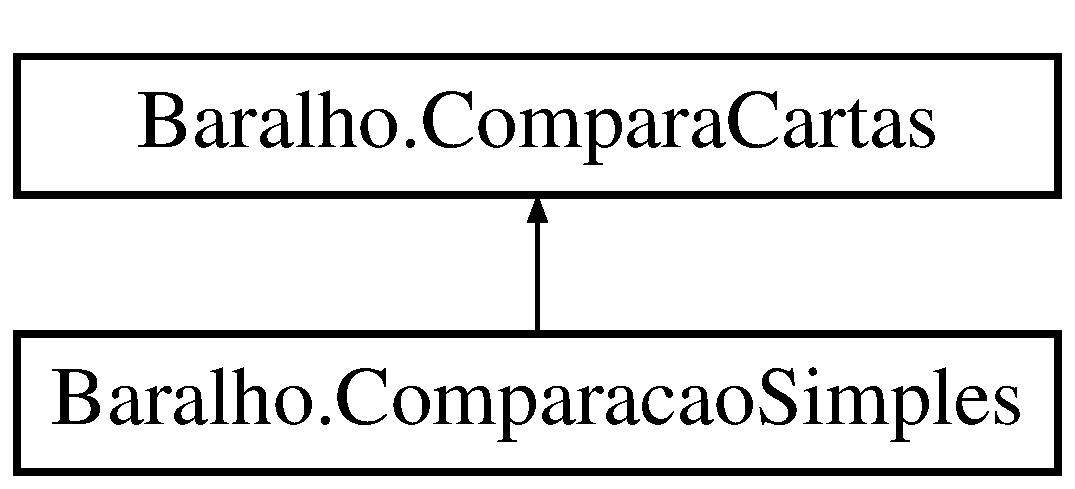
\includegraphics[height=2.000000cm]{class_baralho_1_1_comparacao_simples}
\end{center}
\end{figure}
\subsection*{Public Member Functions}
\begin{DoxyCompactItemize}
\item 
boolean \hyperlink{class_baralho_1_1_comparacao_simples_a1ea37c176e2c216536654b64ac8dc883}{eMaior} (\hyperlink{class_baralho_1_1_carta}{Carta} carta1, \hyperlink{class_baralho_1_1_carta}{Carta} carta2)
\end{DoxyCompactItemize}


\subsection{Detailed Description}
Comparação simples des cartas. \begin{DoxyAuthor}{Author}
Rafael 
\end{DoxyAuthor}


\subsection{Member Function Documentation}
\hypertarget{class_baralho_1_1_comparacao_simples_a1ea37c176e2c216536654b64ac8dc883}{
\index{Baralho::ComparacaoSimples@{Baralho::ComparacaoSimples}!eMaior@{eMaior}}
\index{eMaior@{eMaior}!Baralho::ComparacaoSimples@{Baralho::ComparacaoSimples}}
\subsubsection[{eMaior}]{\setlength{\rightskip}{0pt plus 5cm}boolean Baralho.ComparacaoSimples.eMaior (
\begin{DoxyParamCaption}
\item[{{\bf Carta}}]{carta1, }
\item[{{\bf Carta}}]{carta2}
\end{DoxyParamCaption}
)}}
\label{class_baralho_1_1_comparacao_simples_a1ea37c176e2c216536654b64ac8dc883}
Comparação simples para saber se uma carta tem peso maior que outra. 
\begin{DoxyParams}{Parameters}
{\em carta1} & -\/ \hyperlink{class_baralho_1_1_carta}{Carta} 1 para comparação. \\
\hline
{\em carta2} & -\/ \hyperlink{class_baralho_1_1_carta}{Carta} 2 para comparação. \\
\hline
\end{DoxyParams}
\begin{DoxyReturn}{Returns}
true -\/ se a carta 1 tiver peso maior que a carta 2. false -\/ se a carta 1 tiver peso menor ou igual que a carta 2. 
\end{DoxyReturn}


Implements \hyperlink{interface_baralho_1_1_compara_cartas_a805a502954c21d6fac410506bf81c955}{Baralho.ComparaCartas}.



The documentation for this class was generated from the following file:\begin{DoxyCompactItemize}
\item 
aula/111450026/Trabalho Baralho/Baralho/src/Baralho/\hyperlink{_comparacao_simples_8java}{ComparacaoSimples.java}\end{DoxyCompactItemize}

\hypertarget{interface_baralho_1_1_compara_cartas}{
\section{Baralho.ComparaCartas Interface Reference}
\label{interface_baralho_1_1_compara_cartas}\index{Baralho::ComparaCartas@{Baralho::ComparaCartas}}
}
Inheritance diagram for Baralho.ComparaCartas:\begin{figure}[H]
\begin{center}
\leavevmode
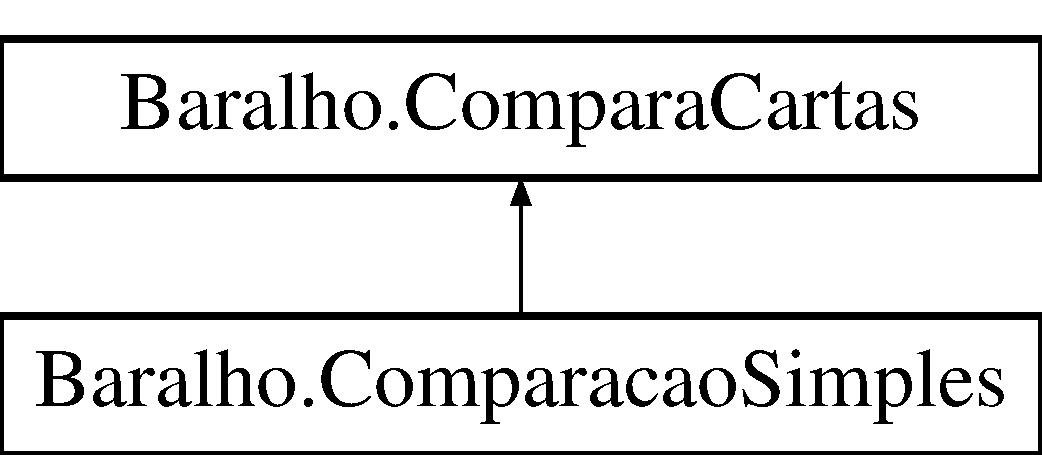
\includegraphics[height=2.000000cm]{interface_baralho_1_1_compara_cartas}
\end{center}
\end{figure}
\subsection*{Public Member Functions}
\begin{DoxyCompactItemize}
\item 
boolean \hyperlink{interface_baralho_1_1_compara_cartas_a805a502954c21d6fac410506bf81c955}{eMaior} (\hyperlink{class_baralho_1_1_carta}{Carta} carta1, \hyperlink{class_baralho_1_1_carta}{Carta} carta2)
\end{DoxyCompactItemize}


\subsection{Detailed Description}
Interface responsável pela comparação das cartas. \begin{DoxyAuthor}{Author}
Rafael 
\end{DoxyAuthor}


\subsection{Member Function Documentation}
\hypertarget{interface_baralho_1_1_compara_cartas_a805a502954c21d6fac410506bf81c955}{
\index{Baralho::ComparaCartas@{Baralho::ComparaCartas}!eMaior@{eMaior}}
\index{eMaior@{eMaior}!Baralho::ComparaCartas@{Baralho::ComparaCartas}}
\subsubsection[{eMaior}]{\setlength{\rightskip}{0pt plus 5cm}boolean Baralho.ComparaCartas.eMaior (
\begin{DoxyParamCaption}
\item[{{\bf Carta}}]{carta1, }
\item[{{\bf Carta}}]{carta2}
\end{DoxyParamCaption}
)}}
\label{interface_baralho_1_1_compara_cartas_a805a502954c21d6fac410506bf81c955}
Compara duas cartas pra saber se uma é maior do que a outra. 
\begin{DoxyParams}{Parameters}
{\em carta1} & -\/ \hyperlink{class_baralho_1_1_carta}{Carta} 1 da comparação. \\
\hline
{\em carta2} & -\/ \hyperlink{class_baralho_1_1_carta}{Carta} 2 da comparação. \\
\hline
\end{DoxyParams}
\begin{DoxyReturn}{Returns}
true -\/ se a carta 1 tiver peso maior. false -\/ se a carta 2 tiver peso menor. 
\end{DoxyReturn}


Implemented in \hyperlink{class_baralho_1_1_comparacao_simples_a1ea37c176e2c216536654b64ac8dc883}{Baralho.ComparacaoSimples}.



The documentation for this interface was generated from the following file:\begin{DoxyCompactItemize}
\item 
aula/111450026/Trabalho Baralho/Baralho/src/Baralho/\hyperlink{_compara_cartas_8java}{ComparaCartas.java}\end{DoxyCompactItemize}

\hypertarget{class_baralho_1_1_monte}{
\section{Baralho.Monte Class Reference}
\label{class_baralho_1_1_monte}\index{Baralho::Monte@{Baralho::Monte}}
}
Inheritance diagram for Baralho.Monte:\begin{figure}[H]
\begin{center}
\leavevmode
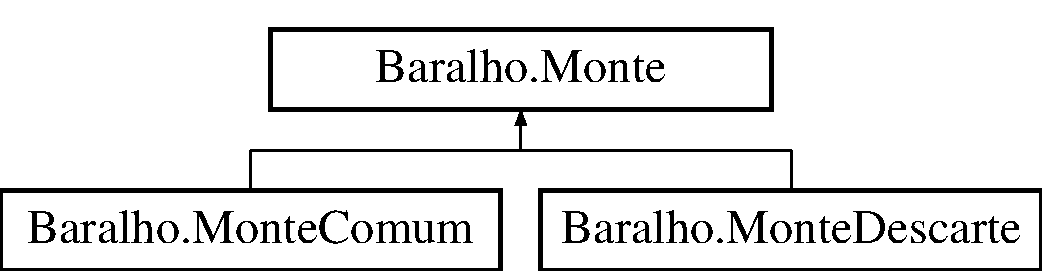
\includegraphics[height=2.000000cm]{class_baralho_1_1_monte}
\end{center}
\end{figure}
\subsection*{Public Member Functions}
\begin{DoxyCompactItemize}
\item 
void \hyperlink{class_baralho_1_1_monte_a9c0e60ff3e5adee7c73311dc639b726d}{initialize} (LinkedList$<$ \hyperlink{class_baralho_1_1_carta}{Carta} $>$ cartas)
\item 
boolean \hyperlink{class_baralho_1_1_monte_a62727fc8f2a5df78acf7ed256907d18d}{addCarta} (\hyperlink{class_baralho_1_1_carta}{Carta} carta)
\item 
void \hyperlink{class_baralho_1_1_monte_a54573fe9edbac3f8d9fca1fe1199debb}{addCarta} (\hyperlink{class_baralho_1_1_carta}{Carta} carta, int pos)  throws IndexOutOfBoundsException
\item 
void \hyperlink{class_baralho_1_1_monte_a64abc4bdca4718cb5e615154c562cf85}{removeCarta} (\hyperlink{class_baralho_1_1_carta}{Carta} carta)  throws CartaInexistenteException
\item 
void \hyperlink{class_baralho_1_1_monte_a81b0e1160db4914f5b1ba51fc068b1b9}{removeCarta} (int pos)  throws CartaInexistenteException 
\item 
LinkedList$<$ \hyperlink{class_baralho_1_1_carta}{Carta} $>$ \hyperlink{class_baralho_1_1_monte_a586ca35231a6c8a8634600df898f5ccc}{listaCartas} ()
\item 
\hyperlink{class_baralho_1_1_carta}{Carta} \hyperlink{class_baralho_1_1_monte_adeda515ad018d4975fbf054a37ab0f36}{obtemCarta} (int pos)  throws CartaInexistenteException
\item 
\hyperlink{class_baralho_1_1_carta}{Carta} \hyperlink{class_baralho_1_1_monte_ad724ab32986fbbc07e3d492aecfa2037}{obtemCarta} (\hyperlink{class_baralho_1_1_carta}{Carta} carta)  throws CartaInexistenteException 
\item 
void \hyperlink{class_baralho_1_1_monte_abd353fab5c3bfe77a070aafe7d905bec}{esvaziaMonte} ()
\item 
int \hyperlink{class_baralho_1_1_monte_a8768f18eb0e16b7a2be665360ad4afb5}{tamanho} ()
\end{DoxyCompactItemize}


\subsection{Detailed Description}
Classe abstrata que representa um monte do baralho. As posições das cartas do monte são consideradas de baixo para cima. \begin{DoxyAuthor}{Author}
Rafael 
\end{DoxyAuthor}


\subsection{Member Function Documentation}
\hypertarget{class_baralho_1_1_monte_a62727fc8f2a5df78acf7ed256907d18d}{
\index{Baralho::Monte@{Baralho::Monte}!addCarta@{addCarta}}
\index{addCarta@{addCarta}!Baralho::Monte@{Baralho::Monte}}
\subsubsection[{addCarta}]{\setlength{\rightskip}{0pt plus 5cm}boolean Baralho.Monte.addCarta (
\begin{DoxyParamCaption}
\item[{{\bf Carta}}]{carta}
\end{DoxyParamCaption}
)}}
\label{class_baralho_1_1_monte_a62727fc8f2a5df78acf7ed256907d18d}
Adiciona uma carta ao monte. 
\begin{DoxyParams}{Parameters}
{\em carta} & -\/ \hyperlink{class_baralho_1_1_carta}{Carta} a ser adicionda. \\
\hline
\end{DoxyParams}
\begin{DoxyReturn}{Returns}
true se a carta foi adicionada ou false caso contrário. 
\end{DoxyReturn}
\hypertarget{class_baralho_1_1_monte_a54573fe9edbac3f8d9fca1fe1199debb}{
\index{Baralho::Monte@{Baralho::Monte}!addCarta@{addCarta}}
\index{addCarta@{addCarta}!Baralho::Monte@{Baralho::Monte}}
\subsubsection[{addCarta}]{\setlength{\rightskip}{0pt plus 5cm}void Baralho.Monte.addCarta (
\begin{DoxyParamCaption}
\item[{{\bf Carta}}]{carta, }
\item[{int}]{pos}
\end{DoxyParamCaption}
)  throws IndexOutOfBoundsException}}
\label{class_baralho_1_1_monte_a54573fe9edbac3f8d9fca1fe1199debb}
Adiciona uma carta em uma posição específica do monte. 
\begin{DoxyParams}{Parameters}
{\em carta} & -\/ \hyperlink{class_baralho_1_1_carta}{Carta} a ser adicionada. \\
\hline
{\em pos} & -\/ Posição onde a carta será inserida. \\
\hline
\end{DoxyParams}

\begin{DoxyExceptions}{Exceptions}
{\em IndexOutOfBoundsException} & -\/ caso a posição em que a carta for inserida for fora dos limites do monte (menor que 0 ou maior que o tamanho do baralho). \\
\hline
\end{DoxyExceptions}
\hypertarget{class_baralho_1_1_monte_abd353fab5c3bfe77a070aafe7d905bec}{
\index{Baralho::Monte@{Baralho::Monte}!esvaziaMonte@{esvaziaMonte}}
\index{esvaziaMonte@{esvaziaMonte}!Baralho::Monte@{Baralho::Monte}}
\subsubsection[{esvaziaMonte}]{\setlength{\rightskip}{0pt plus 5cm}void Baralho.Monte.esvaziaMonte (
\begin{DoxyParamCaption}
{}
\end{DoxyParamCaption}
)}}
\label{class_baralho_1_1_monte_abd353fab5c3bfe77a070aafe7d905bec}
Retira todas as cartas do monte. \hypertarget{class_baralho_1_1_monte_a9c0e60ff3e5adee7c73311dc639b726d}{
\index{Baralho::Monte@{Baralho::Monte}!initialize@{initialize}}
\index{initialize@{initialize}!Baralho::Monte@{Baralho::Monte}}
\subsubsection[{initialize}]{\setlength{\rightskip}{0pt plus 5cm}void Baralho.Monte.initialize (
\begin{DoxyParamCaption}
\item[{LinkedList$<$ {\bf Carta} $>$}]{cartas}
\end{DoxyParamCaption}
)}}
\label{class_baralho_1_1_monte_a9c0e60ff3e5adee7c73311dc639b726d}
Inicializa o monte. As cartas que haviam nele são excluídas. 
\begin{DoxyParams}{Parameters}
{\em cartas} & -\/ Cartas do monte. \\
\hline
\end{DoxyParams}
\hypertarget{class_baralho_1_1_monte_a586ca35231a6c8a8634600df898f5ccc}{
\index{Baralho::Monte@{Baralho::Monte}!listaCartas@{listaCartas}}
\index{listaCartas@{listaCartas}!Baralho::Monte@{Baralho::Monte}}
\subsubsection[{listaCartas}]{\setlength{\rightskip}{0pt plus 5cm}LinkedList$<${\bf Carta}$>$ Baralho.Monte.listaCartas (
\begin{DoxyParamCaption}
{}
\end{DoxyParamCaption}
)}}
\label{class_baralho_1_1_monte_a586ca35231a6c8a8634600df898f5ccc}
Retorna as cartas do monte. \begin{DoxyReturn}{Returns}
-\/ cartas do monte. 
\end{DoxyReturn}
\hypertarget{class_baralho_1_1_monte_ad724ab32986fbbc07e3d492aecfa2037}{
\index{Baralho::Monte@{Baralho::Monte}!obtemCarta@{obtemCarta}}
\index{obtemCarta@{obtemCarta}!Baralho::Monte@{Baralho::Monte}}
\subsubsection[{obtemCarta}]{\setlength{\rightskip}{0pt plus 5cm}{\bf Carta} Baralho.Monte.obtemCarta (
\begin{DoxyParamCaption}
\item[{{\bf Carta}}]{carta}
\end{DoxyParamCaption}
)  throws {\bf CartaInexistenteException} }}
\label{class_baralho_1_1_monte_ad724ab32986fbbc07e3d492aecfa2037}
Retorna uma carta do monte. 
\begin{DoxyParams}{Parameters}
{\em carta} & -\/ A carta que se deseja obter do monte. \\
\hline
\end{DoxyParams}
\begin{DoxyReturn}{Returns}
A carta que se deseja, se ela constar no monte, ou null, caso contrário. 
\end{DoxyReturn}

\begin{DoxyExceptions}{Exceptions}
{\em CartaInexistenteException} & -\/ Caso a carta especificada não conste no monte. \\
\hline
\end{DoxyExceptions}
\hypertarget{class_baralho_1_1_monte_adeda515ad018d4975fbf054a37ab0f36}{
\index{Baralho::Monte@{Baralho::Monte}!obtemCarta@{obtemCarta}}
\index{obtemCarta@{obtemCarta}!Baralho::Monte@{Baralho::Monte}}
\subsubsection[{obtemCarta}]{\setlength{\rightskip}{0pt plus 5cm}{\bf Carta} Baralho.Monte.obtemCarta (
\begin{DoxyParamCaption}
\item[{int}]{pos}
\end{DoxyParamCaption}
)  throws {\bf CartaInexistenteException}}}
\label{class_baralho_1_1_monte_adeda515ad018d4975fbf054a37ab0f36}
Retorna a carta de uma posição do monte. 
\begin{DoxyParams}{Parameters}
{\em pos} & -\/ posição da carta no monte. \\
\hline
\end{DoxyParams}
\begin{DoxyReturn}{Returns}
A carta, se ela constar no monte, ou null, caso contrário. 
\end{DoxyReturn}

\begin{DoxyExceptions}{Exceptions}
{\em CartaInexistenteException} & -\/ Caso a posição especificada não aponte para uma carta do monte. \\
\hline
\end{DoxyExceptions}
\hypertarget{class_baralho_1_1_monte_a64abc4bdca4718cb5e615154c562cf85}{
\index{Baralho::Monte@{Baralho::Monte}!removeCarta@{removeCarta}}
\index{removeCarta@{removeCarta}!Baralho::Monte@{Baralho::Monte}}
\subsubsection[{removeCarta}]{\setlength{\rightskip}{0pt plus 5cm}void Baralho.Monte.removeCarta (
\begin{DoxyParamCaption}
\item[{{\bf Carta}}]{carta}
\end{DoxyParamCaption}
)  throws {\bf CartaInexistenteException}}}
\label{class_baralho_1_1_monte_a64abc4bdca4718cb5e615154c562cf85}
Remove uma carta do monte. 
\begin{DoxyParams}{Parameters}
{\em carta} & -\/ \hyperlink{class_baralho_1_1_carta}{Carta} a ser removida. \\
\hline
\end{DoxyParams}
\begin{DoxyReturn}{Returns}
true se a carta foi removida ou false caso contrário. 
\end{DoxyReturn}
\hypertarget{class_baralho_1_1_monte_a81b0e1160db4914f5b1ba51fc068b1b9}{
\index{Baralho::Monte@{Baralho::Monte}!removeCarta@{removeCarta}}
\index{removeCarta@{removeCarta}!Baralho::Monte@{Baralho::Monte}}
\subsubsection[{removeCarta}]{\setlength{\rightskip}{0pt plus 5cm}void Baralho.Monte.removeCarta (
\begin{DoxyParamCaption}
\item[{int}]{pos}
\end{DoxyParamCaption}
)  throws {\bf CartaInexistenteException} }}
\label{class_baralho_1_1_monte_a81b0e1160db4914f5b1ba51fc068b1b9}
Remove uma carta do monte. 
\begin{DoxyParams}{Parameters}
{\em pos} & -\/ posição da carta que irá ser removida. \\
\hline
\end{DoxyParams}
\begin{DoxyReturn}{Returns}
true se a carta foi removida ou false caso contrário. 
\end{DoxyReturn}
\hypertarget{class_baralho_1_1_monte_a8768f18eb0e16b7a2be665360ad4afb5}{
\index{Baralho::Monte@{Baralho::Monte}!tamanho@{tamanho}}
\index{tamanho@{tamanho}!Baralho::Monte@{Baralho::Monte}}
\subsubsection[{tamanho}]{\setlength{\rightskip}{0pt plus 5cm}int Baralho.Monte.tamanho (
\begin{DoxyParamCaption}
{}
\end{DoxyParamCaption}
)}}
\label{class_baralho_1_1_monte_a8768f18eb0e16b7a2be665360ad4afb5}
Retorna o tamanho do monte. \begin{DoxyReturn}{Returns}
tamanho do monte. 
\end{DoxyReturn}


The documentation for this class was generated from the following file:\begin{DoxyCompactItemize}
\item 
aula/111450026/Trabalho Baralho/Baralho/src/Baralho/\hyperlink{_monte_8java}{Monte.java}\end{DoxyCompactItemize}

\hypertarget{class_baralho_1_1_monte_comum}{
\section{Baralho.MonteComum Class Reference}
\label{class_baralho_1_1_monte_comum}\index{Baralho::MonteComum@{Baralho::MonteComum}}
}
Inheritance diagram for Baralho.MonteComum:\begin{figure}[H]
\begin{center}
\leavevmode
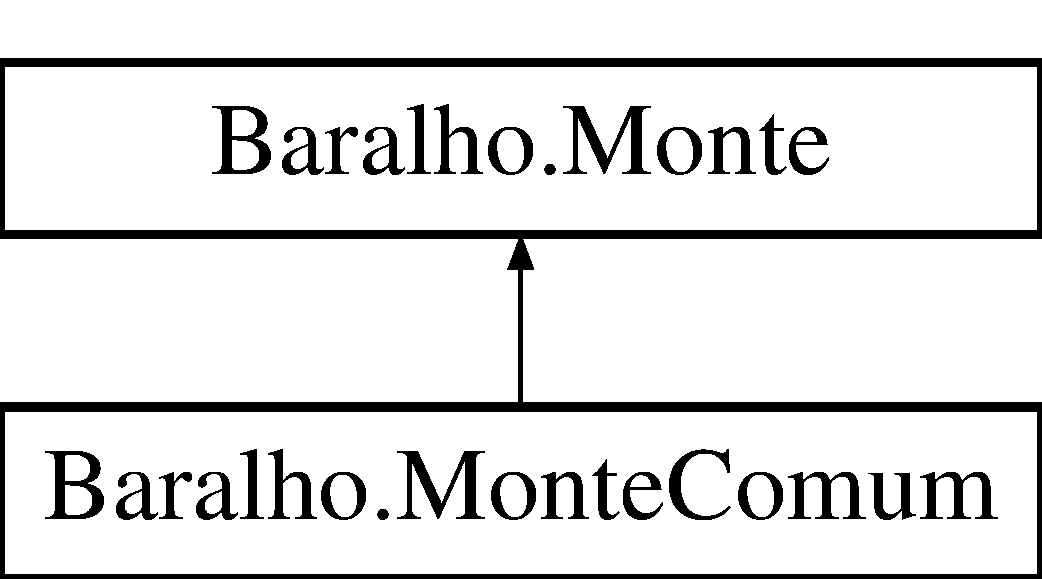
\includegraphics[height=2.000000cm]{class_baralho_1_1_monte_comum}
\end{center}
\end{figure}
\subsection*{Public Member Functions}
\begin{DoxyCompactItemize}
\item 
\hyperlink{class_baralho_1_1_monte_comum_af3664ab9b41ef3ea435033c9ae0132b9}{MonteComum} (LinkedList$<$ \hyperlink{class_baralho_1_1_carta}{Carta} $>$ cartas)
\item 
\hyperlink{class_baralho_1_1_monte_comum_ae5f9907b5ae8ec73544895110c7a0395}{MonteComum} ()
\end{DoxyCompactItemize}


\subsection{Detailed Description}
\hyperlink{class_baralho_1_1_monte}{Monte} comum de cartas. \begin{DoxyAuthor}{Author}
Rafael 
\end{DoxyAuthor}


\subsection{Constructor \& Destructor Documentation}
\hypertarget{class_baralho_1_1_monte_comum_af3664ab9b41ef3ea435033c9ae0132b9}{
\index{Baralho::MonteComum@{Baralho::MonteComum}!MonteComum@{MonteComum}}
\index{MonteComum@{MonteComum}!Baralho::MonteComum@{Baralho::MonteComum}}
\subsubsection[{MonteComum}]{\setlength{\rightskip}{0pt plus 5cm}Baralho.MonteComum.MonteComum (
\begin{DoxyParamCaption}
\item[{LinkedList$<$ {\bf Carta} $>$}]{cartas}
\end{DoxyParamCaption}
)}}
\label{class_baralho_1_1_monte_comum_af3664ab9b41ef3ea435033c9ae0132b9}
Método construtor. Chama initialize da classe monte. 
\begin{DoxyParams}{Parameters}
{\em cartas} & -\/ Cartas iniciais do monte. \\
\hline
\end{DoxyParams}
\hypertarget{class_baralho_1_1_monte_comum_ae5f9907b5ae8ec73544895110c7a0395}{
\index{Baralho::MonteComum@{Baralho::MonteComum}!MonteComum@{MonteComum}}
\index{MonteComum@{MonteComum}!Baralho::MonteComum@{Baralho::MonteComum}}
\subsubsection[{MonteComum}]{\setlength{\rightskip}{0pt plus 5cm}Baralho.MonteComum.MonteComum (
\begin{DoxyParamCaption}
{}
\end{DoxyParamCaption}
)}}
\label{class_baralho_1_1_monte_comum_ae5f9907b5ae8ec73544895110c7a0395}


The documentation for this class was generated from the following file:\begin{DoxyCompactItemize}
\item 
aula/111450026/Trabalho Baralho/Baralho/src/Baralho/\hyperlink{_monte_comum_8java}{MonteComum.java}\end{DoxyCompactItemize}

\hypertarget{class_baralho_1_1_monte_descarte}{
\section{Baralho.MonteDescarte Class Reference}
\label{class_baralho_1_1_monte_descarte}\index{Baralho::MonteDescarte@{Baralho::MonteDescarte}}
}
Inheritance diagram for Baralho.MonteDescarte:\begin{figure}[H]
\begin{center}
\leavevmode
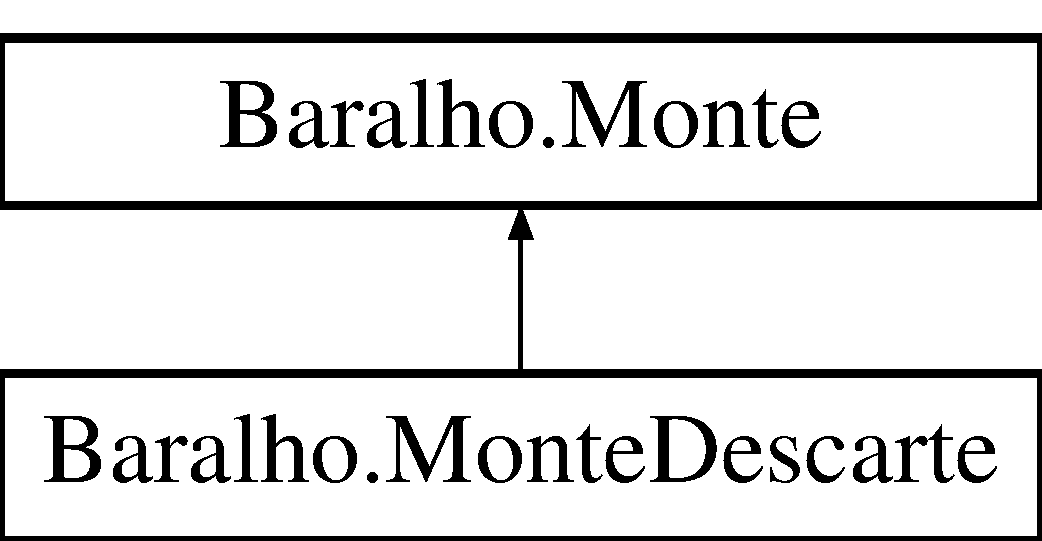
\includegraphics[height=2.000000cm]{class_baralho_1_1_monte_descarte}
\end{center}
\end{figure}
\subsection*{Public Member Functions}
\begin{DoxyCompactItemize}
\item 
\hyperlink{class_baralho_1_1_monte_descarte_a6dad15a6fd2ff4a535663173892936c7}{MonteDescarte} (LinkedList$<$ \hyperlink{class_baralho_1_1_carta}{Carta} $>$ cartas)
\item 
\hyperlink{class_baralho_1_1_monte_descarte_aa36589f9e036fb890115e89e37b3b658}{MonteDescarte} ()
\item 
void \hyperlink{class_baralho_1_1_monte_descarte_a96b713dba347cd79bd944c0bef8a47ae}{exibirCarta} (\hyperlink{class_baralho_1_1_carta}{Carta} carta)
\item 
void \hyperlink{class_baralho_1_1_monte_descarte_a62c26b774387cec5611d723986c78ab0}{exibirCarta} (int pos)
\end{DoxyCompactItemize}


\subsection{Detailed Description}
\hyperlink{class_baralho_1_1_monte}{Monte} de descarte do baralho. Com ele é possível ver cartas sem que sejam retiradas do monte. \begin{DoxyAuthor}{Author}
pc 
\end{DoxyAuthor}


\subsection{Constructor \& Destructor Documentation}
\hypertarget{class_baralho_1_1_monte_descarte_a6dad15a6fd2ff4a535663173892936c7}{
\index{Baralho::MonteDescarte@{Baralho::MonteDescarte}!MonteDescarte@{MonteDescarte}}
\index{MonteDescarte@{MonteDescarte}!Baralho::MonteDescarte@{Baralho::MonteDescarte}}
\subsubsection[{MonteDescarte}]{\setlength{\rightskip}{0pt plus 5cm}Baralho.MonteDescarte.MonteDescarte (
\begin{DoxyParamCaption}
\item[{LinkedList$<$ {\bf Carta} $>$}]{cartas}
\end{DoxyParamCaption}
)}}
\label{class_baralho_1_1_monte_descarte_a6dad15a6fd2ff4a535663173892936c7}
Método construtor. Chama initialize da classe monte. 
\begin{DoxyParams}{Parameters}
{\em cartas} & -\/ Cartas iniciais do monte. \\
\hline
\end{DoxyParams}
\hypertarget{class_baralho_1_1_monte_descarte_aa36589f9e036fb890115e89e37b3b658}{
\index{Baralho::MonteDescarte@{Baralho::MonteDescarte}!MonteDescarte@{MonteDescarte}}
\index{MonteDescarte@{MonteDescarte}!Baralho::MonteDescarte@{Baralho::MonteDescarte}}
\subsubsection[{MonteDescarte}]{\setlength{\rightskip}{0pt plus 5cm}Baralho.MonteDescarte.MonteDescarte (
\begin{DoxyParamCaption}
{}
\end{DoxyParamCaption}
)}}
\label{class_baralho_1_1_monte_descarte_aa36589f9e036fb890115e89e37b3b658}


\subsection{Member Function Documentation}
\hypertarget{class_baralho_1_1_monte_descarte_a96b713dba347cd79bd944c0bef8a47ae}{
\index{Baralho::MonteDescarte@{Baralho::MonteDescarte}!exibirCarta@{exibirCarta}}
\index{exibirCarta@{exibirCarta}!Baralho::MonteDescarte@{Baralho::MonteDescarte}}
\subsubsection[{exibirCarta}]{\setlength{\rightskip}{0pt plus 5cm}void Baralho.MonteDescarte.exibirCarta (
\begin{DoxyParamCaption}
\item[{{\bf Carta}}]{carta}
\end{DoxyParamCaption}
)}}
\label{class_baralho_1_1_monte_descarte_a96b713dba347cd79bd944c0bef8a47ae}
Exibe os dados da carta. 
\begin{DoxyParams}{Parameters}
{\em carta} & -\/ carta a ser exibida. \\
\hline
\end{DoxyParams}
\hypertarget{class_baralho_1_1_monte_descarte_a62c26b774387cec5611d723986c78ab0}{
\index{Baralho::MonteDescarte@{Baralho::MonteDescarte}!exibirCarta@{exibirCarta}}
\index{exibirCarta@{exibirCarta}!Baralho::MonteDescarte@{Baralho::MonteDescarte}}
\subsubsection[{exibirCarta}]{\setlength{\rightskip}{0pt plus 5cm}void Baralho.MonteDescarte.exibirCarta (
\begin{DoxyParamCaption}
\item[{int}]{pos}
\end{DoxyParamCaption}
)}}
\label{class_baralho_1_1_monte_descarte_a62c26b774387cec5611d723986c78ab0}
Exibe os dados da carta. 
\begin{DoxyParams}{Parameters}
{\em pos} & -\/ posição no monte da carta que se deseja exibir. \\
\hline
\end{DoxyParams}


The documentation for this class was generated from the following file:\begin{DoxyCompactItemize}
\item 
aula/111450026/Trabalho Baralho/Baralho/src/Baralho/\hyperlink{_monte_descarte_8java}{MonteDescarte.java}\end{DoxyCompactItemize}

\hypertarget{class_exce_xC3_xA7_xC3_xB5es_1_1_sequencia_invalida_exception}{
\section{Exceções.SequenciaInvalidaException Class Reference}
\label{class_exce_xC3_xA7_xC3_xB5es_1_1_sequencia_invalida_exception}\index{Exceções::SequenciaInvalidaException@{Exceções::SequenciaInvalidaException}}
}
\subsection*{Public Member Functions}
\begin{DoxyCompactItemize}
\item 
\hyperlink{class_exce_xC3_xA7_xC3_xB5es_1_1_sequencia_invalida_exception_af6f229d3f7c1b2faaff12d7a0a71eba1}{SequenciaInvalidaException} (String s)
\item 
String \hyperlink{class_exce_xC3_xA7_xC3_xB5es_1_1_sequencia_invalida_exception_a81cb14dec977306ce54527685ef130fc}{getMessage} ()
\end{DoxyCompactItemize}


\subsection{Detailed Description}
\begin{DoxyAuthor}{Author}
rafael 
\end{DoxyAuthor}


\subsection{Constructor \& Destructor Documentation}
\hypertarget{class_exce_xC3_xA7_xC3_xB5es_1_1_sequencia_invalida_exception_af6f229d3f7c1b2faaff12d7a0a71eba1}{
\index{Exceções::SequenciaInvalidaException@{Exceções::SequenciaInvalidaException}!SequenciaInvalidaException@{SequenciaInvalidaException}}
\index{SequenciaInvalidaException@{SequenciaInvalidaException}!Exceções::SequenciaInvalidaException@{Exceções::SequenciaInvalidaException}}
\subsubsection[{SequenciaInvalidaException}]{\setlength{\rightskip}{0pt plus 5cm}Exceções.SequenciaInvalidaException.SequenciaInvalidaException (
\begin{DoxyParamCaption}
\item[{String}]{s}
\end{DoxyParamCaption}
)}}
\label{class_exce_xC3_xA7_xC3_xB5es_1_1_sequencia_invalida_exception_af6f229d3f7c1b2faaff12d7a0a71eba1}


\subsection{Member Function Documentation}
\hypertarget{class_exce_xC3_xA7_xC3_xB5es_1_1_sequencia_invalida_exception_a81cb14dec977306ce54527685ef130fc}{
\index{Exceções::SequenciaInvalidaException@{Exceções::SequenciaInvalidaException}!getMessage@{getMessage}}
\index{getMessage@{getMessage}!Exceções::SequenciaInvalidaException@{Exceções::SequenciaInvalidaException}}
\subsubsection[{getMessage}]{\setlength{\rightskip}{0pt plus 5cm}String Exceções.SequenciaInvalidaException.getMessage (
\begin{DoxyParamCaption}
{}
\end{DoxyParamCaption}
)}}
\label{class_exce_xC3_xA7_xC3_xB5es_1_1_sequencia_invalida_exception_a81cb14dec977306ce54527685ef130fc}


The documentation for this class was generated from the following file:\begin{DoxyCompactItemize}
\item 
aula/111450026/Trabalho Baralho/Baralho/src/Exceções/\hyperlink{_sequencia_invalida_exception_8java}{SequenciaInvalidaException.java}\end{DoxyCompactItemize}

\chapter{File Documentation}
\hypertarget{_baralho_8java}{
\section{aula/111450026/Trabalho Baralho/Baralho/src/Baralho/Baralho.java File Reference}
\label{_baralho_8java}\index{aula/111450026/Trabalho Baralho/Baralho/src/Baralho/Baralho.java@{aula/111450026/Trabalho Baralho/Baralho/src/Baralho/Baralho.java}}
}
\subsection*{Classes}
\begin{DoxyCompactItemize}
\item 
class \hyperlink{class_baralho_1_1_baralho}{Baralho.Baralho}
\end{DoxyCompactItemize}
\subsection*{Packages}
\begin{DoxyCompactItemize}
\item 
package \hyperlink{namespace_baralho}{Baralho}
\end{DoxyCompactItemize}

\hypertarget{_carta_8java}{
\section{aula/111450026/Trabalho Baralho/Baralho/src/Baralho/Carta.java File Reference}
\label{_carta_8java}\index{aula/111450026/Trabalho Baralho/Baralho/src/Baralho/Carta.java@{aula/111450026/Trabalho Baralho/Baralho/src/Baralho/Carta.java}}
}
\subsection*{Classes}
\begin{DoxyCompactItemize}
\item 
class \hyperlink{class_baralho_1_1_carta}{Baralho.Carta}
\end{DoxyCompactItemize}
\subsection*{Packages}
\begin{DoxyCompactItemize}
\item 
package \hyperlink{namespace_baralho}{Baralho}
\end{DoxyCompactItemize}

\hypertarget{_comparacao_simples_8java}{
\section{aula/111450026/Trabalho Baralho/Baralho/src/Baralho/ComparacaoSimples.java File Reference}
\label{_comparacao_simples_8java}\index{aula/111450026/Trabalho Baralho/Baralho/src/Baralho/ComparacaoSimples.java@{aula/111450026/Trabalho Baralho/Baralho/src/Baralho/ComparacaoSimples.java}}
}
\subsection*{Classes}
\begin{DoxyCompactItemize}
\item 
class \hyperlink{class_baralho_1_1_comparacao_simples}{Baralho.ComparacaoSimples}
\end{DoxyCompactItemize}
\subsection*{Packages}
\begin{DoxyCompactItemize}
\item 
package \hyperlink{namespace_baralho}{Baralho}
\end{DoxyCompactItemize}

\hypertarget{_compara_cartas_8java}{
\section{aula/111450026/Trabalho Baralho/Baralho/src/Baralho/ComparaCartas.java File Reference}
\label{_compara_cartas_8java}\index{aula/111450026/Trabalho Baralho/Baralho/src/Baralho/ComparaCartas.java@{aula/111450026/Trabalho Baralho/Baralho/src/Baralho/ComparaCartas.java}}
}
\subsection*{Classes}
\begin{DoxyCompactItemize}
\item 
interface \hyperlink{interface_baralho_1_1_compara_cartas}{Baralho.ComparaCartas}
\end{DoxyCompactItemize}
\subsection*{Packages}
\begin{DoxyCompactItemize}
\item 
package \hyperlink{namespace_baralho}{Baralho}
\end{DoxyCompactItemize}

\hypertarget{_monte_8java}{
\section{aula/111450026/Trabalho Baralho/Baralho/src/Baralho/Monte.java File Reference}
\label{_monte_8java}\index{aula/111450026/Trabalho Baralho/Baralho/src/Baralho/Monte.java@{aula/111450026/Trabalho Baralho/Baralho/src/Baralho/Monte.java}}
}
\subsection*{Classes}
\begin{DoxyCompactItemize}
\item 
class \hyperlink{class_baralho_1_1_monte}{Baralho.Monte}
\end{DoxyCompactItemize}
\subsection*{Packages}
\begin{DoxyCompactItemize}
\item 
package \hyperlink{namespace_baralho}{Baralho}
\end{DoxyCompactItemize}

\hypertarget{_monte_comum_8java}{
\section{aula/111450026/Trabalho Baralho/Baralho/src/Baralho/MonteComum.java File Reference}
\label{_monte_comum_8java}\index{aula/111450026/Trabalho Baralho/Baralho/src/Baralho/MonteComum.java@{aula/111450026/Trabalho Baralho/Baralho/src/Baralho/MonteComum.java}}
}
\subsection*{Classes}
\begin{DoxyCompactItemize}
\item 
class \hyperlink{class_baralho_1_1_monte_comum}{Baralho.MonteComum}
\end{DoxyCompactItemize}
\subsection*{Packages}
\begin{DoxyCompactItemize}
\item 
package \hyperlink{namespace_baralho}{Baralho}
\end{DoxyCompactItemize}

\hypertarget{_monte_descarte_8java}{
\section{aula/111450026/Trabalho Baralho/Baralho/src/Baralho/MonteDescarte.java File Reference}
\label{_monte_descarte_8java}\index{aula/111450026/Trabalho Baralho/Baralho/src/Baralho/MonteDescarte.java@{aula/111450026/Trabalho Baralho/Baralho/src/Baralho/MonteDescarte.java}}
}
\subsection*{Classes}
\begin{DoxyCompactItemize}
\item 
class \hyperlink{class_baralho_1_1_monte_descarte}{Baralho.MonteDescarte}
\end{DoxyCompactItemize}
\subsection*{Packages}
\begin{DoxyCompactItemize}
\item 
package \hyperlink{namespace_baralho}{Baralho}
\end{DoxyCompactItemize}

\hypertarget{_naipe_8java}{
\section{aula/111450026/Trabalho Baralho/Baralho/src/Baralho/Naipe.java File Reference}
\label{_naipe_8java}\index{aula/111450026/Trabalho Baralho/Baralho/src/Baralho/Naipe.java@{aula/111450026/Trabalho Baralho/Baralho/src/Baralho/Naipe.java}}
}
\subsection*{Packages}
\begin{DoxyCompactItemize}
\item 
package \hyperlink{namespace_baralho}{Baralho}
\end{DoxyCompactItemize}
\subsection*{Enumerations}
\begin{DoxyCompactItemize}
\item 
enum \hyperlink{namespace_baralho_ab887857dcb81ef6672322ce80039b905}{Baralho.Naipe} \{ \hyperlink{namespace_baralho_ab887857dcb81ef6672322ce80039b905}{Baralho.OUROS}, 
\hyperlink{namespace_baralho_ab887857dcb81ef6672322ce80039b905}{Baralho.peso}, 
\hyperlink{namespace_baralho_ab887857dcb81ef6672322ce80039b905}{Baralho.peso}, 
\hyperlink{namespace_baralho_ab887857dcb81ef6672322ce80039b905}{Baralho.peso}
 \}
\end{DoxyCompactItemize}

\hypertarget{_carta_inexistente_exception_8java}{
\section{aula/111450026/Trabalho Baralho/Baralho/src/Exceções/CartaInexistenteException.java File Reference}
\label{_carta_inexistente_exception_8java}\index{aula/111450026/Trabalho Baralho/Baralho/src/Exceções/CartaInexistenteException.java@{aula/111450026/Trabalho Baralho/Baralho/src/Exceções/CartaInexistenteException.java}}
}
\subsection*{Classes}
\begin{DoxyCompactItemize}
\item 
class \hyperlink{class_exce_xC3_xA7_xC3_xB5es_1_1_carta_inexistente_exception}{Exceções.CartaInexistenteException}
\end{DoxyCompactItemize}
\subsection*{Packages}
\begin{DoxyCompactItemize}
\item 
package \hyperlink{namespace_exce_xC3_xA7_xC3_xB5es}{Exceções}
\end{DoxyCompactItemize}

\hypertarget{_carta_invalida_exception_8java}{
\section{aula/111450026/Trabalho Baralho/Baralho/src/Exceções/CartaInvalidaException.java File Reference}
\label{_carta_invalida_exception_8java}\index{aula/111450026/Trabalho Baralho/Baralho/src/Exceções/CartaInvalidaException.java@{aula/111450026/Trabalho Baralho/Baralho/src/Exceções/CartaInvalidaException.java}}
}
\subsection*{Classes}
\begin{DoxyCompactItemize}
\item 
class \hyperlink{class_exce_xC3_xA7_xC3_xB5es_1_1_carta_invalida_exception}{Exceções.CartaInvalidaException}
\end{DoxyCompactItemize}
\subsection*{Packages}
\begin{DoxyCompactItemize}
\item 
package \hyperlink{namespace_exce_xC3_xA7_xC3_xB5es}{Exceções}
\end{DoxyCompactItemize}

\hypertarget{_sequencia_invalida_exception_8java}{
\section{aula/111450026/Trabalho Baralho/Baralho/src/Exceções/SequenciaInvalidaException.java File Reference}
\label{_sequencia_invalida_exception_8java}\index{aula/111450026/Trabalho Baralho/Baralho/src/Exceções/SequenciaInvalidaException.java@{aula/111450026/Trabalho Baralho/Baralho/src/Exceções/SequenciaInvalidaException.java}}
}
\subsection*{Classes}
\begin{DoxyCompactItemize}
\item 
class \hyperlink{class_exce_xC3_xA7_xC3_xB5es_1_1_sequencia_invalida_exception}{Exceções.SequenciaInvalidaException}
\end{DoxyCompactItemize}
\subsection*{Packages}
\begin{DoxyCompactItemize}
\item 
package \hyperlink{namespace_exce_xC3_xA7_xC3_xB5es}{Exceções}
\end{DoxyCompactItemize}

\printindex
\end{document}
